
The first papers I could find showcasing the FEM in geodynamics are listed hereafter
(I arbitrarily stop at 1995):
\cite{gart78}, 
\cite{anbr80}\cite{mera80}\cite{bran80}
\cite{engl82}
\cite{thar85}
\cite{enho86}\cite{mofr86}
\cite{zupa86}
\cite{boww89}
\cite{brau94}
\cite{brbe95}.
I hereunder show a few plots taken from early geodynamics papers.


\begin{center}
\begin{minipage}{0.45\textwidth}
\centering
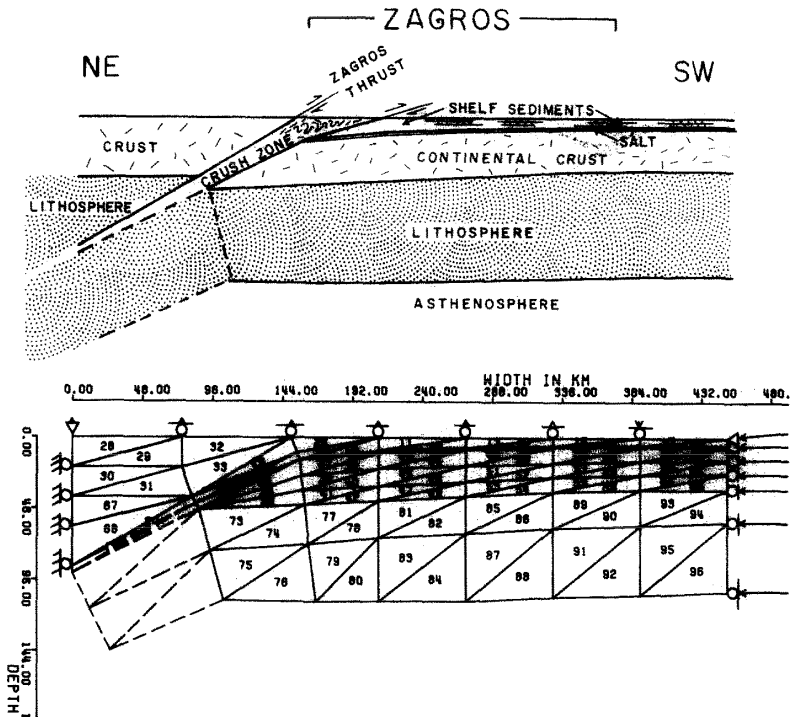
\includegraphics[height=4.5cm]{images/history/bird78b}\\
{\scriptsize 1978: Finite element modelling of lithosphere deformation: the Zagros collision 
orogeny \cite{bird78b}}
\end{minipage}\hfill
\begin{minipage}{0.45\textwidth}
\centering
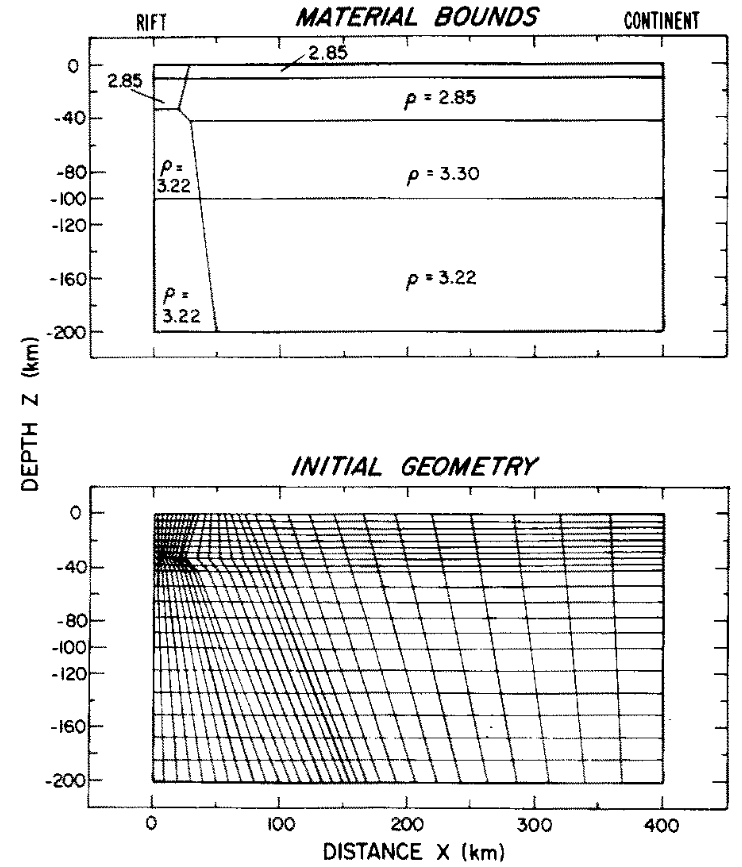
\includegraphics[height=4.5cm]{images/history/brpo81}\\
{\scriptsize 1981: Thermal regimes, mantle diapirs and crustal stresses of continental rifts \cite{brpo81}}
\end{minipage}
\end{center}


\begin{center}
\begin{minipage}{0.48\textwidth}
\centering
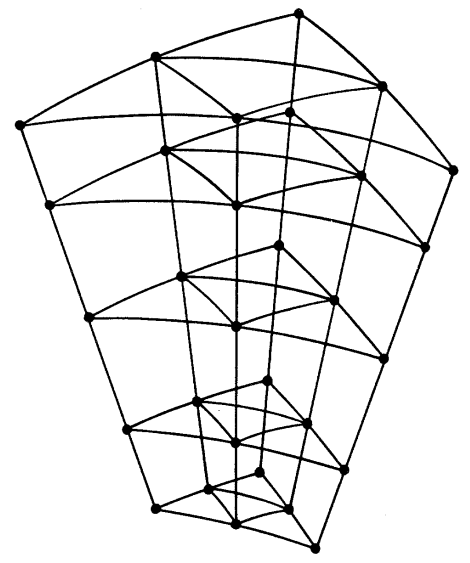
\includegraphics[height=3.5cm]{images/history/baum85a}
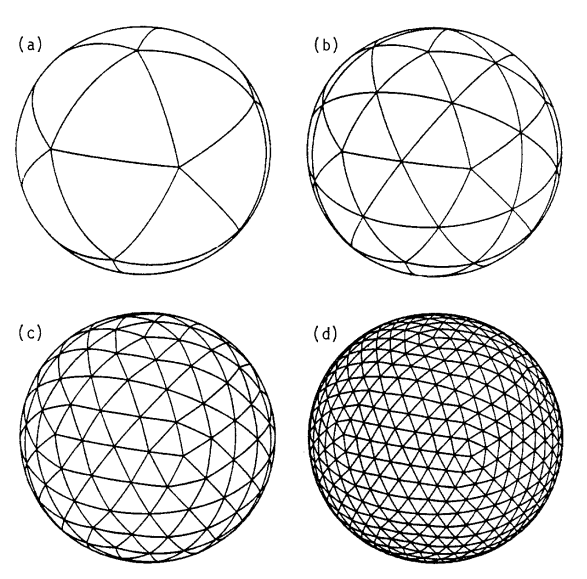
\includegraphics[height=3.5cm]{images/history/baum85b}\\
{\scriptsize 1985: Three-Dimensional Treatment of Convective Flow in the Earth's Mantle.
\cite{baum85}}
\end{minipage}\hfill
\begin{minipage}{0.45\textwidth}
\centering
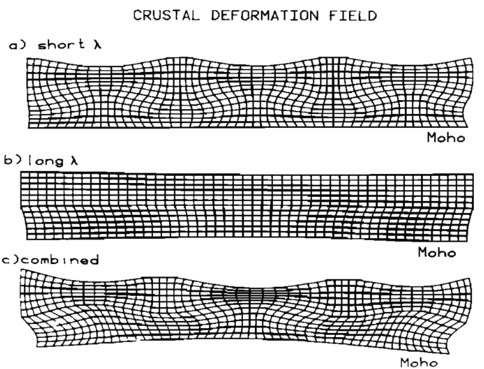
\includegraphics[width=7cm]{images/history/zupf86}\\
{\scriptsize 1986: Lithospheric necking: a dynamic model for rift morphology \cite{zupf86}}
\end{minipage}
\end{center}


\begin{center}
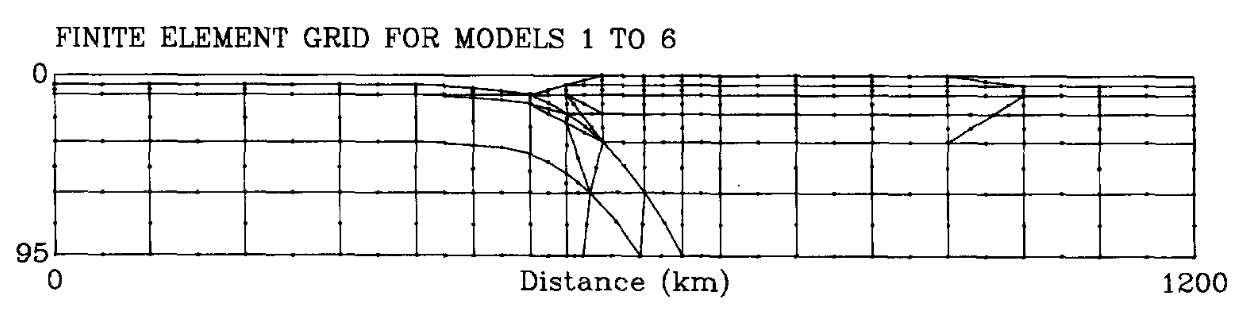
\includegraphics[width=9cm]{images/history/boww89}\\
{\scriptsize 1989: Plate boundary forces at subduction zones and trench-arc compression \cite{boww89}}
\end{center}

\begin{center}
\begin{minipage}{0.35\textwidth}
\centering
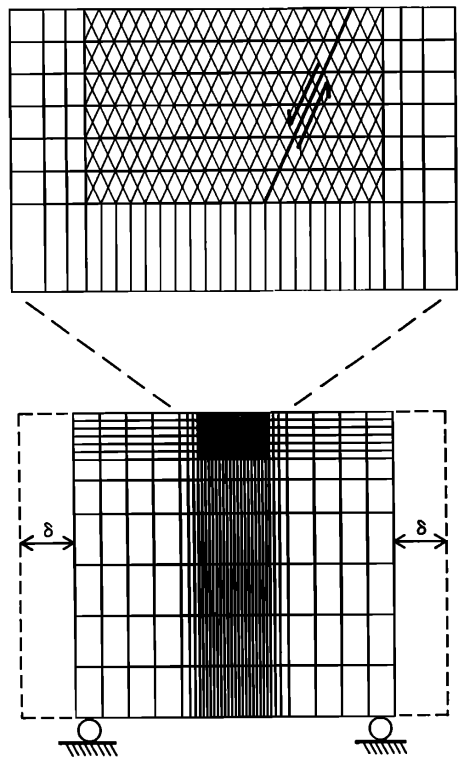
\includegraphics[width=5cm]{images/history/mewi89}\\
{\scriptsize 1989: Mechanics of graben formation in crustal rocks \cite{mewi89}}
\end{minipage}\hfill
\begin{minipage}{0.55\textwidth}
\centering
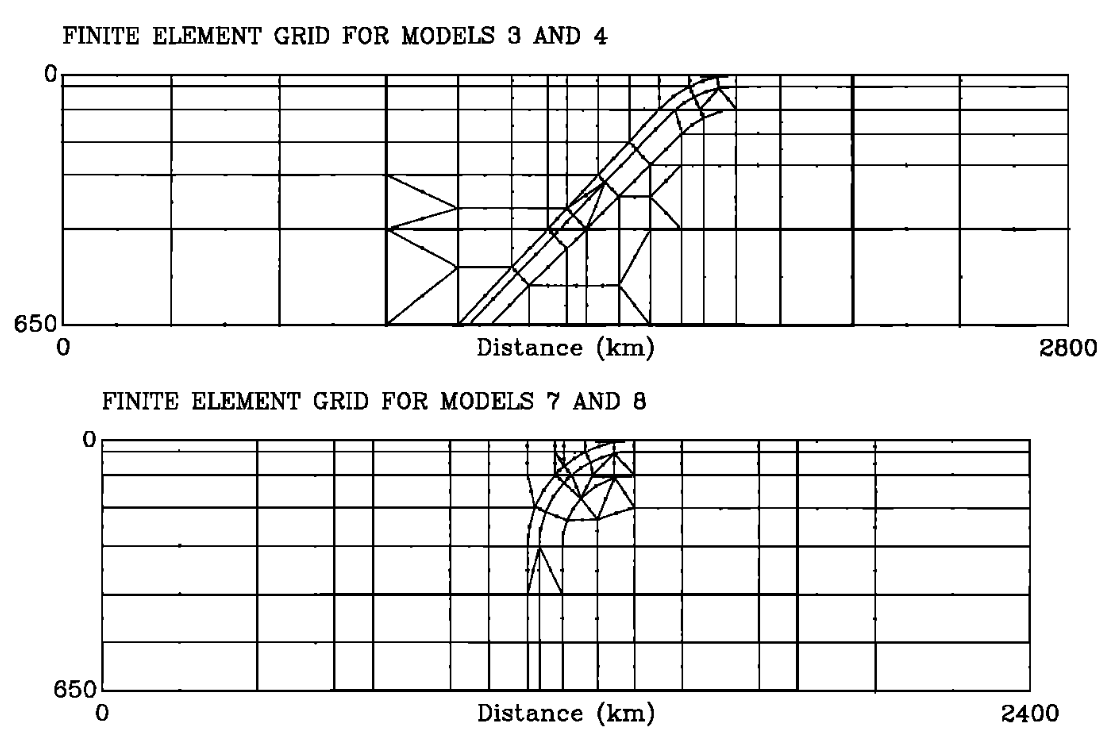
\includegraphics[width=8cm]{images/history/whbw92}\\
{\scriptsize 1992: Stresses and plate boundary forces associated with subduction plate margins
\cite{whbw92}}
\end{minipage}
\end{center}


\begin{center}
\begin{minipage}{0.45\textwidth}
\centering
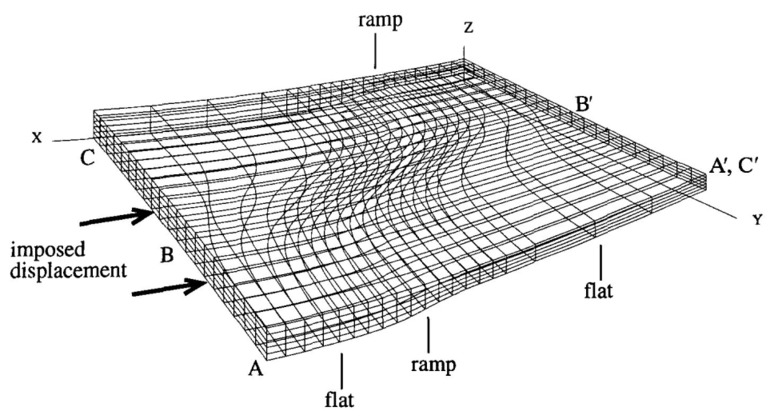
\includegraphics[width=7cm]{images/history/brau93}\\
{\scriptsize 1993: 3D numerical modeling of
compressional orogenies: Thrust geometry and
oblique convergence \cite{brau93}}
\end{minipage}\hfill
\begin{minipage}{0.45\textwidth}
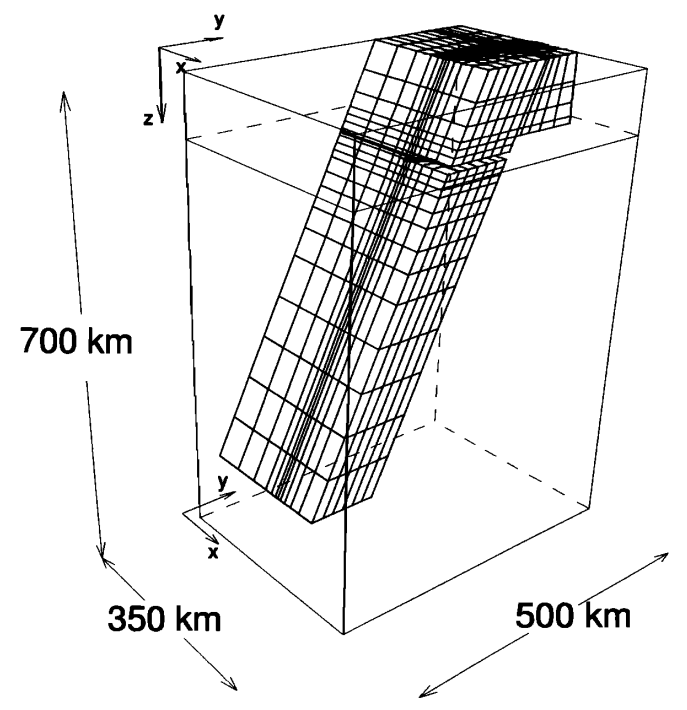
\includegraphics[height=5cm]{images/history/yowo95}\\
{\scriptsize 1995: 3D numerical modeling of detachment of subducted 
lithosphere \cite{yowo95}}
\centering
\end{minipage}
\end{center}



\begin{center}
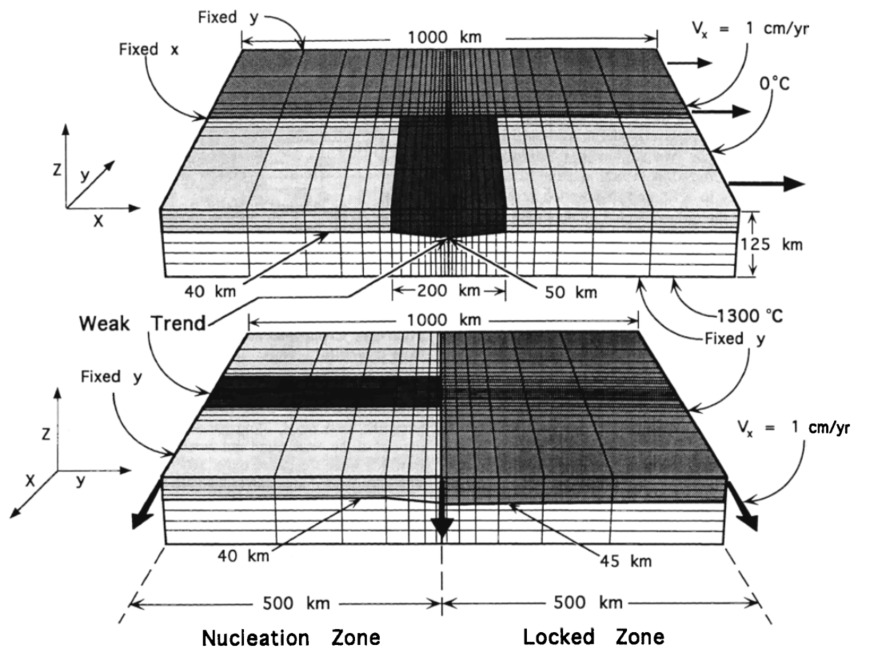
\includegraphics[height=6cm]{images/history/dusa96}\\
{\scriptsize 1996: 3D dynamical model of continental rift propagation and 
margin plateau formation \cite{dusa96}}
\end{center}


